\documentclass{article}
\usepackage{polski}
\usepackage[utf8]{inputenc}

\usepackage{amsthm}
\usepackage{amssymb}
\usepackage{amsmath}
\usepackage{etoolbox}
\usepackage{hyperref}
\usepackage{graphicx} %do grafik
\usepackage{float}

\graphicspath{ {obrazki/} }


\theoremstyle{definition}%
\newtheorem{defn}{Definicja}

\theoremstyle{theorem}
\newtheorem{zad}{Zadanie}
\AfterEndEnvironment{zad}{\noindent\ignorespaces}

\newtheorem{theo}{Stwierdzenie}

\renewenvironment{proof}{{\bfseries Rozwiązanie}}{\qed}


\title{Topologia *}
\author{Mateusz Zugaj, Michal Zmyslowski}
\date{Listopad 2017}w


%Skrócone oznaczenia
\newcommand{\R}{\mathbb{R}} %Zbiór liczb rzeczywistych
\newcommand{\Pow}{\mathcal{P}} %Zbiór potęgowy
\newcommand{\sT}{\mathcal{T}} %Topologia


\begin{document}
	
	\maketitle
	\begin{defn}[Topologie na prostej] W zbiorze liczb rzeczywistych  $\R$ zdefiniujmy rodziny podzbiorów~${\cal T}_i$:
		\begin{enumerate}
			\item ${\cal T}_1=\Pow (\R)$ -- topologia dyskretna
			\item ${\cal T}_2=\{U\subset \R\colon  \forall_{s\in U}\exists_{t>s}[s,t)\subset U\}$ -- topologia prawej strzałki
			\item ${\cal T}_3=\{U\subset \R\colon  \forall_{s\in U}\exists_{t<s}(t,s]\subset U\}$ -- topologia lewej strzałki
			\item ${\cal T}_4=\{U\subset \R\colon  \forall_{s\in U}\exists_{r<s<t}(r,t)\subset U\}$  -- topologia euklidesowa
			\item ${\cal T}_5=\{\emptyset\}\cup\{\R\}\cup\{(-\infty,x)\colon x\in \R\}$ - topologia lewych przedziałów
			\item ${\cal T}_6=\{\emptyset\}\cup\{\R\}\cup\{(x,+\infty)\colon x\in \R\}$ - topologia prawych przedziałów
			\item ${\cal T}_7=\{\emptyset\}\cup\{\R\}\cup\{U\subset \R\colon  \R\setminus U \; \hbox{jest zbiorem skończonym}\}$ -- topologia Zariskiego
			\item ${\cal T}_8=\{\emptyset\}\cup\{\R\}$ -- topologia antydyskretna
		\end{enumerate}
	\end{defn}
	
	\begin{zad}
		Niech $\mathcal{T}_{i}$ będą rodzinami podzbiorów prostej rzeczywistej opisanymi w Definicji 1.\\
		a) Sprawdź, że rodziny $\mathcal{T}_{i}$ są topologiami.\\
		b) Porównaj topologie $\mathcal{T}_{i}$, rysując diagram inkluzji tych Topologii i zbadaj ich przecięcia.\\
		c) Zbadaj, które topologie $\mathcal{T}_{i}$ mają własność Hausdorffa.\\
		d) O których parach przestrzeni $(\mathbb{R},\mathcal{T}_{i})$,$(\mathbb{R},\mathcal{T}_{j})$ potrafisz powiedzieć, że są lub nie są homeomorficzne? Narysuj i wypełnij tabelkę.
	\end{zad}
	\begin{proof}
	b) Ewidentnie $\mathcal{T}_{2}\subset\mathcal{T}_{1}$ i $\mathcal{T}_{3}\subset\mathcal{T}_{1}$. Następnie $[0,1)\in\mathcal{T}_{2}$, ale $[0,1)\not\in\mathcal{T}_{3}$. Podobnie $(0,1]\in\mathcal{T}_{3}$, ale $(0,1]\not\in\mathcal{T}_{2}$. Mamy, że $(0,1)\in\mathcal{T}_{4}$, jak również $(0,1)\in\mathcal{T}_{3}$ i $(0,1)\in\mathcal{T}_{2}$. Jednak $[0,1)\not\in\mathcal{T}_{4}$ i $(0,1]\not\in\mathcal{T}_{4}$. Czyli $\mathcal{T}_{4}\subset\mathcal{T}_{2}$ i $\mathcal{T}_{4}\subset\mathcal{T}_{3}$. Teraz $(-\infty,1)\in\mathcal{T}_{5}$, jak również $(-\infty,1)\in\mathcal{T}_{4}$. Podobnie $(1, \infty)\in\mathcal{T}_{6}$ i $(1, \infty)\in\mathcal{T}_{4}$. Jednak $(0,1)\not\in\mathcal{T}_{5}$ i $(0,1)\not\in\mathcal{T}_{6}$. Tak więc, $\mathcal{T}_{5}\subset\mathcal{T}_{4}$ i $\mathcal{T}_{6}\subset\mathcal{T}_{4}$. Mamy $(-\infty,1)\not\in\mathcal{T}_{7}$ i $(1, \infty)\not\in\mathcal{T}_{7}$. Teraz $\mathbb{R}\setminus\{1\}\in\mathcal{T}_{7}$, ale $\mathbb{R}\setminus\{1\}\not\in\mathcal{T}_{5}$ i $\mathbb{R}\setminus\{1\}\not\in\mathcal{T}_{6}$. Jednak $\mathbb{R}\setminus\{1\}\in\mathcal{T}_{4}$. Czyli $\mathcal{T}_{7}\subset\mathcal{T}_{4}$. Ostatecznie $\mathcal{T}_{8}\subset\mathcal{T}_{5}$, $\mathcal{T}_{8}\subset\mathcal{T}_{6}$,
	$\mathcal{T}_{8}\subset\mathcal{T}_{7}$.
	c) Weźmy dowolne $x,y\in\mathbb{R}$ takie, że $x<y$. Teraz $\mathcal{T}_{1}$ ma własność Hausdorffa, bo $\{x\},\{y\}\in\mathcal{T}_{1}$. Następnie dobierzmy $s,t,r\in\mathbb{R}$, że $x\in(s,t)$ i $y\in(t,r)$. Teraz  $(s,t)\in\mathcal{T}_{4}$ i $(t,r)\in\mathcal{T}_{4}$. Więc $\mathcal{T}_{2}$, $\mathcal{T}_{3}$ i $\mathcal{T}_{4}$ mają własność Hausdorffa.
	Przestrzenie $\mathcal{T}_{i}$ dla $i=5,6,7,8$ nie mają własności Hausdorffa.\\
	d) Od razu można powiedzieć, że każda $\mathcal{T}_{i}$ dla $i=1,2,3,4$ nie jest homeomorficzna z żadną z $\mathcal{T}_{j}$ dla $j=5,6,7,8$, bo wcześniejsze mają własność Hausdorffa, a późniejsze nie. Również $\mathcal{T}_{1}$ nie jest homeomorficzna z $\mathcal{T}_{8}$, bo moc pierwszej jest większa od drugiej, co wiadomo ze Wstępu do Matematyki.
	\end{proof}
	
	\begin{zad} [Bukiet prostych] Niech $J$ będzie dowolnym zbiorem. W zbiorze $\R\times J$ rozpatrzmy relację równoważności $$(t,i)\sim (s,j)\quad\text{wtedy i tylko wtedy gdy}\quad t=s=0\quad\text{lub} \quad (t,i) = (s,j)$$ a zbiór klas abstrakcji oznaczmy  $\R\wedge J^+$. Zauważmy, że $\R\wedge J^+ = \R\times J/0\times J$ tzn. powstaje z iloczynu  $\R\times J$ przez utożsamienie do punktu podzbioru $0\times J$. W zbiorze $\R\wedge J^+$ rozpatrzymy dwie topologie:
		\begin{enumerate} 
			\item Topologię $\sT_k$ wyznaczoną przez metrykę węzła $d_k((t,i),(s,j)) = \begin{cases}  |t-s|\, \text{jeśli}\, i=j \\ |t|+|s|\, \text{jeśli}\, i\neq j\end{cases}$
			
			\item Topologię słabą $\sT_w$  tzn. taką, że zbiór $U\subset \R\wedge J^+$ jest otwarty wtedy i tylko wtedy gdy dla każdego $i\in J$ zbiór $U\cap \R\times\{i\}$ jest otwarty w topologii euklidesowej prostej. 
		\end{enumerate}
		Zauważ, że 
		\begin{enumerate}
			\item $\sT_k\subset \sT_w$
			\item Jeśli $|J|\geq \aleph_0$, to topologia słaba nie spełnia pierwszego aksjomatu przeliczalności.
			\item Jeśli $|J|\geq \aleph_0$, to topologia słaba jest niemetryzowalna.
		\end{enumerate} 
		 \end{zad}
		 \begin{proof}
		 	\begin{enumerate}
		 		\item Niech $U \in \sT_k$. Zauważmy, że kule $B((x,i),r)$ w metryce $d_k$ występują w dwóch postaciach
		 		\begin{enumerate}
		 			\item $B((x,i),r)$ dla $r\leq|x|$ jest odcinkiem otwartym na i-tej prostej, tj. \[
		 			B((x,i),r) \cap \left(\R \times {i}\right) = \underbrace{(x-r,x+r)}_{\text{przedział otwarty!}} \times \{i\}\]
		 			\begin{figure}[H]
		 			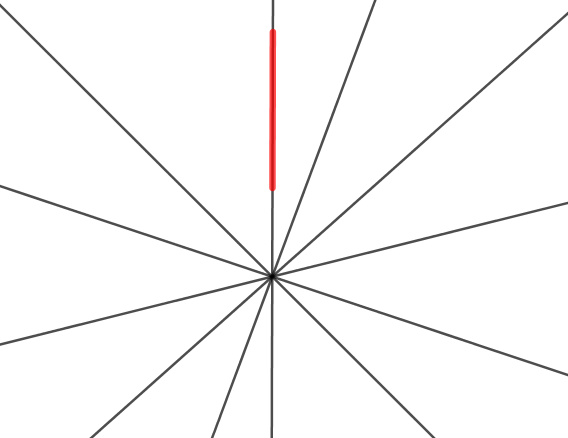
\includegraphics{zad_toposlaba1}
		 			\centering
		 			\end{figure}
		 			\item Dla $r > |x|$ jest to suma dwóch zbiorów, odcinka otwartego zdefiniowanego tak samo jak wyżej ["patyczka"] 
		 			\[
		 			B((x,i),r) \cap \left(\R \times {i}\right) = \underbrace{(x-r,x+r)}_{\text{przedział otwarty!}} \times \{i\}\]
		 			oraz zbioru ["lizaka"]
		 			\[
		 			(-(r-|x|),r-|x|)\times \left(J \setminus \{i\}\right)
		 			\]
		 		
		 	\begin{figure}[H]
		 		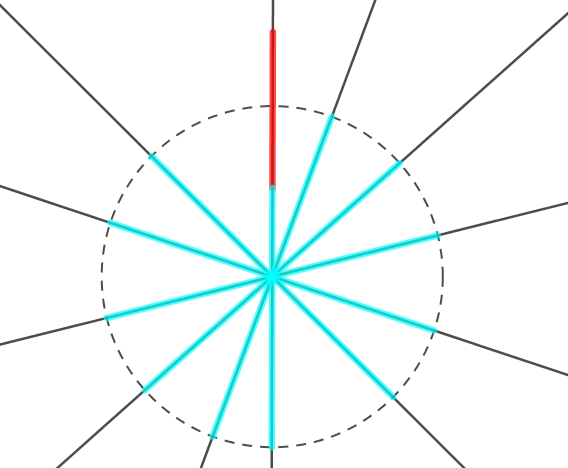
\includegraphics{zad_toposlaba2}
		 		\centering
		 	\end{figure}
		 		\end{enumerate}
		 		Z definicji przestrzeni wyznaczanej przez metrykę każdy zbiór otwarty jest sumą kul w tej metryce, tj. $U=\bigcup_{u\in U } B_u$, gdzie $B_u = B(u,r)$ są zawarte w $U$. \\
		 		Chcemy pokazać, że $U\in \sT_w$, czyli że dla każdego $i$ zbiór $U\cap \left( \R\times\{i\}\right)$ jest otwarty w topologii euklidesowej. Skoro $U = \bigcup B_u$ to wystarczy, że $B_u$ będzie otwarte w $\sT_w$ - wtedy $U$ jako suma zbiorów otwartych w $\sT_w$ będzie otwarta. \\
		 		Ale każda kula jest otwarta w $\sT_w$. Dla dowolnej zachodzi 
		 		\[
		 		B((x,j),r) \cap \left(\R \times \{i\}\right) = \begin{cases}
		 		(x-r,x+r) & r < |x| \vee j = i \\
		 		(-(r-|x|),r-|x|) & r \geq |x| \wedge j \neq i
		 		
		 		\end{cases}
		 		\]
			 	W każdym przypadku, iloczyn jest przedziałem otwartym w topologii euklidesowej. Zatem $B((x,j),r) \in \sT_w$, więc $U\in \sT_w$ zgodnie z tym co wcześniej ustaliliśmy.
			 	\item 
		 		Udowodnimy, że topologia słaba nie ma punktowej bazy przeliczalnej w 0. \\
		 		Załóżmy, że istnieje taka baza $= \{U_1,U_2,U_3,\cdots\}$. Niech $J_0 \subseteq J$ będzie zbiorem przeliczalnym w $J$ i $J_0=\{j_1,j_2,\cdots\}$. Skonstruujemy taki zbiór otwarty $U$, że $0\in V$ ale $\forall k\in \mathbb{N} \; U_k \not\subseteq V$.
		 		Mianowicie bierzemy zbiory
		 		\[
		 		V_k \subsetneq U_k \cap \left(\R \times \{j_k\}\right)
		 		\]
		 		I teraz $V=\bigcup V_k \cup \left((J\setminus J_0)\times \R\right)$. Widzimy, że gdyby $U_k \subseteq V$, to musiałoby być $U_k\cap (\R \times \{j_k\}) \subseteq V \cap (\R \times \{j_k\}) = V_k$, co jest sprzeczne z definicji $V_k$. Zatem założenie o istnieniu bazy przeliczalnej w zerze jest fałszywe.
		 		\item
		 		Gdyby przestrzeń była metryzowalna, to zbiór kul o promieniach wymiernych o środku w 0 byłaby bazą punktową przeliczalną w zerze, co przy tych założeniach jest niemożliwe na mocy poprzedniego podpunktu.
		 	\end{enumerate}
		 	
		 \end{proof}
	
	\begin{zad}
		Niech $d_i$ dla $i = 1,2$ będą dwoma metrykami w zbiorze X. Następujące warunki są równoważne:\\
		1. Topologia wyznaczona przez $d_2$ jest drobniejsza niż wyznaczona przez $d_1$, tzn. $\mathcal{T}(d_1)\subset\mathcal{T}(d_2)$.\\
		2. Dla każdej kuli $\mathcal{B}_{d_1}(x,r_1)$ istnieje liczba $r_2>0$ taka, że $\mathcal{B}_{d_2}(x,r_2)\subset\mathcal{B}_{d_1}(x,r_1)$.\\
		3. Jeśli ciąg jest zbieżny w metryce $d_2$ to jest zbieżny w metryce $d_1$ do tej samej granicy.
			\end{zad}
		\begin{proof}
		\\	$1\implies2$\\
		Załóżmy, że $\mathcal{T}(d_1)\subset\mathcal{T}(d_2)$. Niech $\mathcal{B}_{d_1}(x,r_1)\in\mathcal{T}(d_1)$. Z założenia $\mathcal{B}_{d_1}(x,r_1)\in\mathcal{T}(d_2)$. Z definicji topologii $\mathcal{T}(d_2)$ istnieje $r_2>0$ takie, że\\
		$\mathcal{B}_{d_2}(x,r_2)\subset\mathcal{B}_{d_1}(x,r_1)$.\\
		$2\implies1$\\
		Załóżmy, że  dla każdej kuli $\mathcal{B}_{d_1}(x,r_1)$ istnieje liczba $r_2>0$ taka, że\\ $\mathcal{B}_{d_2}(x,r_2)\subset\mathcal{B}_{d_1}(x,r_1)$. Weźmy dowolny $y_s\in\mathcal{B}_{d_1}(x,r_1)$. Z definicji topologii $\mathcal{T}(d_1)$ istnieje $r>0$ takie, że $\mathcal{B}_{d_1}(y_s,r)\subset\mathcal{B}_{d_1}(x,r_1)$. Z założenia istnieje $r_s>0$ takie, że $\mathcal{B}_{d_2}(y_s,r_s)\subset\mathcal{B}_{d_1}(y_s,r)$. Z tego wynika, że $\bigcup_s \mathcal{B}_{d_2}(y_s,r_s) = \mathcal{B}_{d_1}(x,r_1)\in\mathcal{T}(d_1)$. Z definicji topologii $\bigcup_s \mathcal{B}_{d_2}(y_s,r_s)\in\mathcal{T}(d_2)$. Tak, więc $\mathcal{T}(d_1)\subset\mathcal{T}(d_2)$.\\
		$1\implies3$\\
		Załóżmy, że $\mathcal{T}(d_1)\subset\mathcal{T}(d_2)$. Niech ciąg $\{x_n\}_{n=1}^\infty$ będzie zbieżny do $x$ w metryce $d_2$. Załóżmy, że $\{x_n\}_{n=1}^\infty$ nie jest zbieżny do $x$ w metryce $d_1$. Z tego wynika, że istnieje $\epsilon>0$, taki, że dla każdego $n_{\epsilon}$ istnieje $n>n_{\epsilon}$, że $x_n\not\in\mathcal{B}_{d_1}(x,\epsilon)$. Z założenia $\mathcal{T}(d_1)\subset\mathcal{T}(d_2)$ wynika jednak, że istnieje liczba $r>0$ taka, że $\mathcal{B}_{d_2}(x,r)\subset\mathcal{B}_{d_1}(x,\epsilon)$. Jako, że $\{x_n\}_{n=1}^\infty$ jest zbieżny do $x$ w metryce $d_2$, to z definicji zbieżności prawie wszystkie wyrazy $\{x_n\}_{n=1}^\infty$ znajdują się w $\mathcal{B}_{d_2}(x,r)$, co jest sprzeczne z faktem, że $x_n\not\in\mathcal{B}_{d_1}(x,\epsilon)$. Z tego wynika, że $\{x_n\}_{n=1}^\infty$ jest zbieżny do $x$ w metryce $d_1$.\\
		$3\implies1$\\
		Załóżmy, że jeśli ciąg jest zbieżny w metryce $d_2$ to jest zbieżny w metryce $d_1$. Zawieranie się topologii jest równoważne zawieraniu się rodziny zbiorów domkniętych, tzn. $\mathcal{F}_{\mathcal{T}(d_1)}\subset\mathcal{F}_{\mathcal{T}(d_2)}\Longleftrightarrow\mathcal{T}(d_1)\subset\mathcal{T}(d_2)$. Udowodnimy ten fakt w "prawą" stronę. Niech $A\in\mathcal{F}_{\mathcal{T}(d_1)}$. Jako, że $A$ jest zbiorem domkniętym to $X\setminus A$ jest zbiorem otwartym, więc $X\setminus A\in\mathcal{T}(d_1)$. Z założenia wynika, że $A\in\mathcal{F}_{\mathcal{T}(d_2)}$, więc również $X\setminus A\in\mathcal{T}(d_2)$. Niech $M\in\mathcal{F}_{\mathcal{T}(d_1)}$. Z definicji domknięcia dostajemy, że $M\subset cl_{\mathcal{T}(d_2)}(M)$. Jeżeli $x\in cl_{\mathcal{T}(d_2)}(M)$, to istnieje $\{x_n\}_{n=1}^\infty \subset M$, taki, że $d_2(x_n,x)\to 0$. Z założenia dostajemy, że $d_1(x_n,x)\to 0$. Z tego wynika, że $x\in cl_{\mathcal{T}(d_1)}(M)$. M jest domknięty w $\mathcal{T}(d_1)$, czyli $M=cl_{\mathcal{T}(d_1)}(M)$. A z tego mamy, że $x\in M$, co daje
		$cl_{\mathcal{T}(d_2)}(M)\subset M$. Wtedy $cl_{\mathcal{T}(d_2)}(M)=M$, a z tego wynika, że $M\in \mathcal{F}_{\mathcal{T}(d_2)}$, czyli  $\mathcal{F}_{\mathcal{T}(d_1)}\subset \mathcal{F}_{\mathcal{T}(d_2)}$. Tak więc, na mocy faktu, który wcześniej udowodniliśmy $\mathcal{T}(d_1)\subset\mathcal{T}(d_2)$.\\
		\end{proof}

	\begin{defn}
		Niech $(X,\mathcal{T})$ będzie przestrzenią topologiczną. Przez $C(X)$ oznaczamy zbiór
		funkcji ciągłych $f:(X,\mathcal{T}) \to (\mathbb{R},\mathcal{T}_{e})$, a przez $C_{b}(X)$ jego podzbiór składający się z funkcji ograniczonych. Dla dowolnej funkcji $f \in C_{b}(X)$ definiujemy $\|f\|_{sup}:=sup\{|f(x)|:x \in X\}$ oraz $\|f\|_{L^1}:=\int_0^1 |f(t)| dt$.
	\end{defn}
	\begin{zad}
		Porównać topologię wyznaczoną przez normę $\|f\|_{sup}$ z topologią wyznaczoną przez normę $\|f\|_{L^1}$.
	\end{zad}
	\begin{proof}
	Niech
	\[f_{n}(x):= \begin{cases} 
	1-nx\ ,\ x \in [0,\frac{1}{n}]\\
	0\ ,\ x \in (\frac{1}{n},1)
	\end{cases}\] Wtedy  $f_{n} \in C_{b}([0,1])$ i  $\|f_{n}(x)\|_{L^1}=\frac{1}{2n} \to 0$, ale
	$\|f_{n}(x)\|_{sup}=1 \not\to 0$.\\
	Rozważmy $g_{n} \in C_{b}([0,1])$ taką, że $\|g_{n}(x)\|_{sup} \to 0$.
	Wtedy na mocy \href[page=220]{skryptAM1.pdf}{9.31} $\|g_{n}(x)\|_{L^1}\leq$ $sup(|g_{n}(x)|)(1-0)\to 0$.\\
	Niech $d_{sup}(f,g)=\|f-g\|_{sup}$ i $d_{L^1}(f,g)=\|f-g\|_{L^1}$.
	Rozpatrzmy $(C_{b}(X), d_{sup})$  i $(C_{b}(X), d_{L^1})$. Jeżeli $f_n$ jest zbieżny do f w przestrzeni $(C_{b}(X), d_{sup})$, tzn. $d_{sup}(f_n,f)\to0$, to z wcześniejszych obserwacji $d_{L^1}(f_n,f)\to0$, czyli jest zbieżny, również do f, w $(C_{b}(X), d_{L^1})$. Z poprzedniego zadania wiemy już, że wtedy $\mathcal{T}(d_{L^1})\subset\mathcal{T}(d_{sup})$.
	\end{proof}
\end{document}%